\documentclass[crop=false]{standalone}

\begin{document}
	\section{Expected Result}
	本文實驗假設無人機在固定高度,固定速度下前進,並且給定三個參數,1) 給定無人機初始座標位置,2) 給定終點目標 3)隨機生成多個障礙物後,將障礙物位置當成第二個輸入參數。我們預期在獲得輸入參數後,無人機起飛後會首先調整前進方向,由於本文假設無人機以固定速度前進,只需要持續計算與障礙物的距離,並且與障礙物保持安全距離,以及調整方向在並避開障礙物的同時也保持朝向終點方向前進。總結來說,我們預期透過使用DWA方法,無人機將能夠避開障礙物,並以穩定的速度行向自目的地, 如圖1所示:
    
    \begin{figure}[htbp]	
    	\centering
    	\begin{minipage}{0.49\linewidth}
    		\centering
    		\fbox{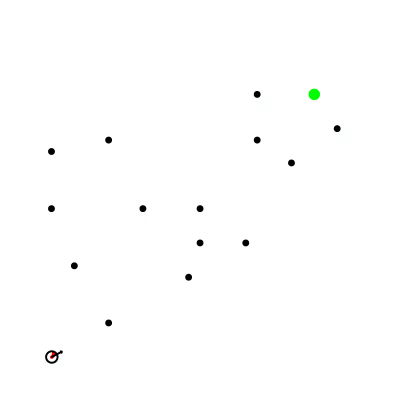
\includegraphics[width=0.9\linewidth]{dwa_frame_0.png}}
    		\caption{Initial point}
    		\label{Initial robot point}%文中引用该图片代号
    	\end{minipage}
    	\begin{minipage}{0.49\linewidth}
    		\centering
    		\fbox{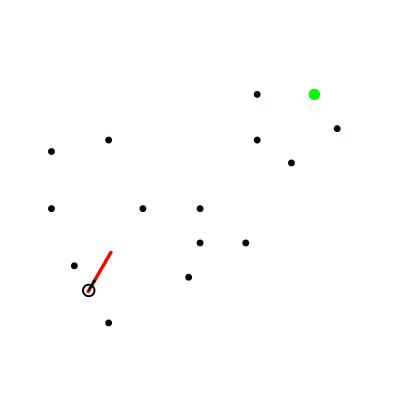
\includegraphics[width=0.9\linewidth]{dwa_frame_1.png}}
    		\caption{Robot is moving}
    		\label{Moving robot}%文中引用该图片代号
    	\end{minipage}
    	%\qquad
    	%让图片换行,
    	
    	\begin{minipage}{0.49\linewidth}
    		\centering
    		\fbox{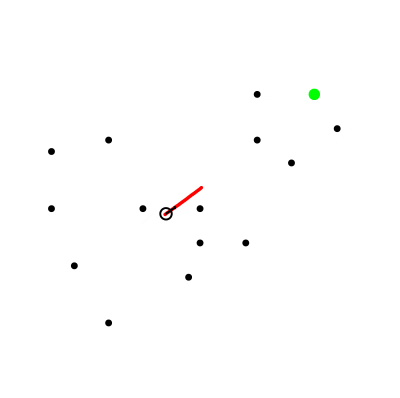
\includegraphics[width=0.9\linewidth]{dwa_frame_2.png}}
    		\caption{Robot avoid obstacles}
    		\label{Robot avoid obstacles}%文中引用该图片代号
    	\end{minipage}
    	\begin{minipage}{0.49\linewidth}
    		\centering
    		\fbox{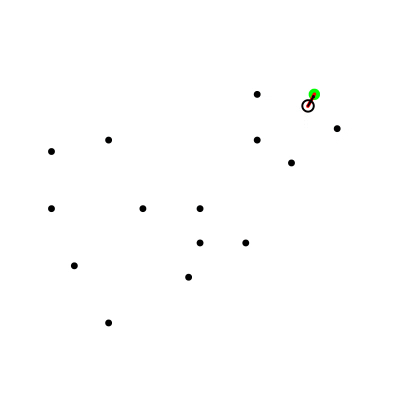
\includegraphics[width=0.9\linewidth]{dwa_frame_3.png}}
    		\caption{Robot is arrived target point}
    		\label{Robot is arrived target point}%文中引用该图片代号
    	\end{minipage}
    \end{figure}
\end{document}

